\section{研究背景}
\subsection{问题背景}
\begin{frame}
\frametitle{问题背景}
\begin{columns}
\begin{column}[b]{0.35\textwidth}
\begin{center}
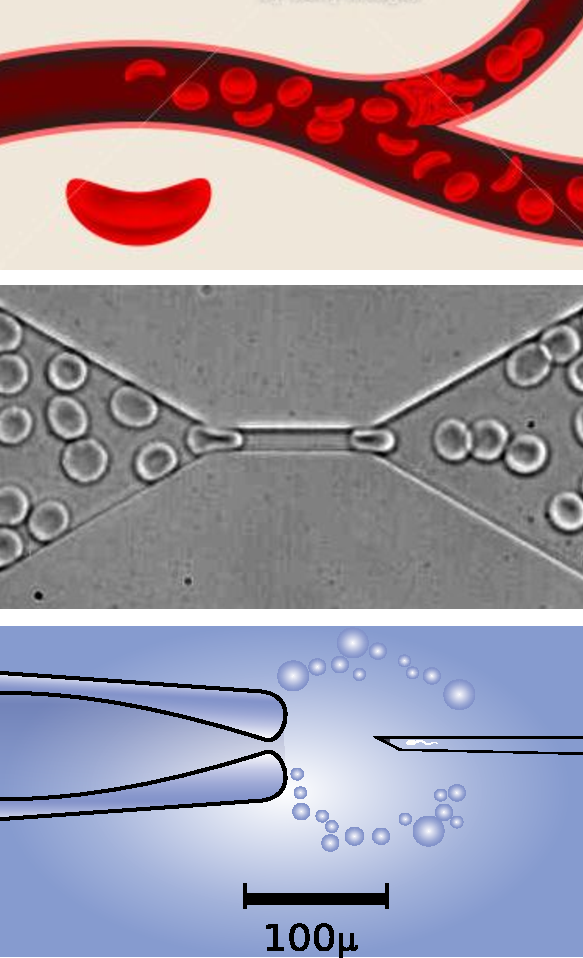
\includegraphics[width=0.9\textwidth]{microdivice.pdf}
\end{center}
\end{column}
\begin{column}[b]{0.65\textwidth}
复杂流体往往涉及多元, 多相, 多组分, 一般难以用牛顿流体模型描述. 复杂流体多尺度流动现象普遍存在于生命科学, 环境工程, 生化工程和微纳米科技等不同领域.\note{\textcolor{red}{[15-45s]}复杂流体的多尺度流动普遍存在于生命科学, 环境工程等不同领域.}
\begin{itemize}
\item 生物体内的体液流动, 包括毛细血管内的血液流动, 关系到生物体的健康. 
     \note[item]{比如毛细血管内的血液流动}
\item 生物微流动器件利用细胞的力学差异对正常细胞与病变细胞进行区分.
     \note[item]{微吸管法利用微流动判断和区分细胞是否病变}
\item 微针利用微流动可以高效而精确的对细胞, 局部组织等进行微小剂量的药物或高分子的输送. 
     \note[item]{微针利用微流动进行的卵胞浆内单精子注射.}
\end{itemize}
\end{column}
\end{columns}
\end{frame}

\subsection{研究现状}
\begin{frame}
\frametitle{不同尺度的方法}
\begin{figure}
\includegraphics<1>[width=\textwidth]{spatiotemporal.pdf}
\includegraphics<2>[width=\textwidth]{spatiotemporal1.pdf}
\includegraphics<3>[width=\textwidth]{spatiotemporal2.pdf}
\includegraphics<4>[width=\textwidth]{spatiotemporal3.pdf}
\note{\textcolor{red}{[45-100s]}对于不同尺度的问题,需要相应尺度的方法.}
\note<2->[item]{对于微观尺度的问题, 可以用分子动力学, 甚至量子计算来模拟. 分子动力学由于计算尺度的限制, 很难对介观尺度以上的流动进行模拟.}
\note<3->[item]{对于宏观问题, 可以用基于连续介质假设的NS方程来模拟. 当问题所涉及的空间尺度逐渐缩小到介观乃至微观时, NS方程就未必适用.}
\note<4->[item]{对于介于微观和宏观尺度, 我们称为介观, 常用的介观尺度的方法有耗散粒子动力学, 布勆动力学等方法. 布朗动力学等不大适合模拟处理含生物高分子, 细胞等的复杂流体行为. 最终我们选择了耗散粒子动力学方法.}
\end{figure}
\end{frame}

%\begin{frame}
%\frametitle{常用方法的不足}
%复杂流体的多尺度计算模型涉及从微观到介观甚至宏观尺度的时间和空间流体动力学特征.
%\note{\textcolor{red}{[100-130s]}我们研究的对象主要是介观尺度流动现象, 直接相关的物理特性往往处于毫秒, 微米级, 因此介于纳米与毫米之间的介观尺度模拟方法合理选择.}
%\begin{itemize}
%\item 传统的网格方法一般基于连续介质力学假设, 当问题所涉及的空间尺度逐渐缩小到介观乃至微观时未必适用. 
%     \note[item]{传统的网格方法一般基于连续介质力学假设, 对于介观乃至微观的问题未必适用.}
%\item 由于当前计算条件的限制,分子动力学模拟所涉及的时间及空间尺度还仅限于纳秒和纳米级,很难对介观尺度以上的流动区域进行模拟. 
%     \note[item]{而分子动力学方向又因为计算尺度的限制, 很难对介观尺度以上的流动进行模拟.}
%\item 作为介观尺度的方法, 布朗动力学, 格子气自动机及网格波尔兹曼等不大适合模拟处理含生物高分子, 细胞等的复杂流体行为.
%     \note[item]{作为观尺度的方法, 布朗动力学, 格子气自动机等不大适合模拟处理含生物高分子, 细胞等的复杂流体行为.}
%\end{itemize}
%\end{frame}
